\documentclass[12pt]{amsart}
\usepackage[utf8]{inputenc}
\usepackage[a4paper, total={6in, 8.5in}]{geometry}
\usepackage{amsmath}
\usepackage{upgreek}
\usepackage{amssymb}
\usepackage{amsrefs}
\usepackage{bm}
\usepackage{fancyhdr}
\usepackage{graphicx}
\usepackage{caption}

\newlength\mystoreparindent
\newenvironment{myparindent}[1]{%
\setlength{\mystoreparindent}{\the\parindent}
\setlength{\parindent}{#1}
}{%
\setlength{\parindent}{\mystoreparindent}
}
 
\pagestyle{fancy}
\fancyhf{}
\rhead{Google Summer of Code Proposal}
\lhead{Taras Kolomatski}

\title{ACTS: CPU Race for Particle Hunting}
\date{\vspace{-1.0cm}Taras Kolomatski}

\usepackage{titling}
\setlength{\droptitle}{-6em}
\parskip 0.2cm 

\usepackage{geometry}
\usepackage{xcolor}
\usepackage[colorlinks = true, urlcolor  = blue]{hyperref}
\geometry{outer=2.5cm,inner=2.5cm}

\begin{document}

\maketitle

\thispagestyle{empty}

\vspace{-0.4cm}

\section*{Introduction}

Experimental particle physics is as a process of reconstruction, as direct detection of the physical phenomena of interest is sometimes impossible. For example, the Higgs boson has a mean lifetime of $10^{-22}$ seconds, which theoretically limits the expected distance it can travel to $3 \times 10^{-14}$ metres - far too short to reach a detector's sensitive elements. What is detected are changes in the statistical patterns of the particles that we do measure, originating from the Higgs boson's decay products. However, there are also limitations to the information we can extract from particles that do reach a detector's sensitive elements. For example, we are not able to accurately measure the momentum of electrically neutral particles. Roughly, the game is approximately as follows: we tabulate the measurements that we can, infer missing terms from conservation laws, piece together which particles could give those terms, and finally perform a statistical analysis to infer that certain decays occurred.

Long-lived charged particles are a rich source of information as we can track the curves that they follow under a strong magnetic field. Inner layers of the detector are sensitive media that respond to, but do not significantly impede, the particles that cross them. Thus, the data we obtain are several snapshots of points on this curve, to some error bars, followed by the energy deposition pattern of particles in the calorimeter, an outer layer which stops most of them. By disrupting the particles more significantly, this outer layer is able to make observations that the inner tracking layers do not. The process of recovering the path followed by particles in the inner tracking layers is called track reconstruction. It involves first analysing the inner layers and making a guess at which curves could give rise to that collection of points, and then testing these predictions against the measurements made in the outer layers.

\begin{figure}[h]
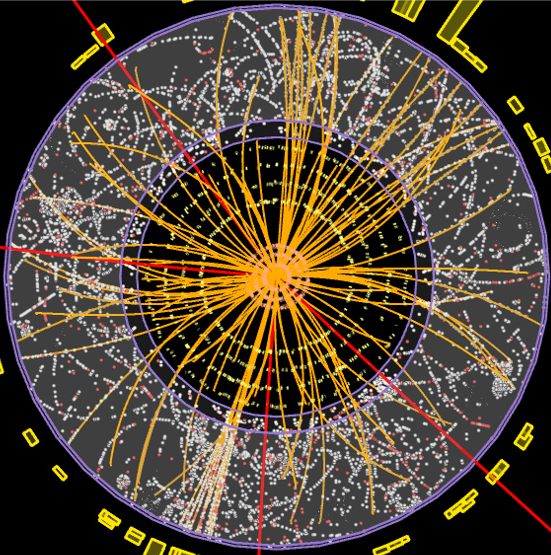
\includegraphics[scale=0.3]{ATLAS}
\caption*{Track predictions fit against observation at the ATLAS detector in the LHC.}
\centering
\end{figure}

ACTS is an open source library aiming to provide experiment-agnostic tools for track reconstruction, building on the successful statistical methods in the software of previous experiments. Such data analysis software was previously highly experiment-specific. The adoption of efficient universally used libraries is critical as although upcoming accelerator upgrades (e.g. HL-LHC and FCC) are expected to result in orders of magnitude increase in data set sizes, public funding shortages on experimental fundamental physics research result in the prediction that data analysis costs will stand at at 10x budget overrun.

\section*{The Proposal}

I will work on a part of the ACTS codebase that implements the non-linear Kalman filter algorithm, used for preliminary fitting (simulating and testing of track hypotheses). Track hypotheses live in a five dimensional parameter space, and the implementation makes heavy use of linear algebra on symmetric $5 \times 5$ matrices. Many of the steps involve independently applying some operation to a large collection of matrices, and is hence amenable to vectorisation by use of SIMD instructions. Additionally, the symmetric $5 \times 5$ case necessarily admits optimisations that are not efficient for square matrices of larger size.

ACTS chose the \texttt{Eigen} library for its linear algebra needs, which benchmarking showed to be a clear choice among its contenders. However, even this library's handling of low-dimensional matrices remains imperfect. Matrix operations are merely translated into loops which the compiler is expected automatically vectorise, but may not, leading to large performance fluctuations across compiler configurations. And the library's algorithms have not been particularly optimised for efficient handling of smaller matrices.

Previously, a research intern with the ACTS team made a processor specific low level implementation of square matrix multiplication and inversion algorithms which demonstrated a substantial improvement over the program produced by \texttt{Eigen}. They produced the following table in the case of inversion. It represents time taken to invert $10^7$ matrices as compared with \texttt{Eigen}, on two different compiler optimisation settings (-O3 and -Ofast).

\begin{figure}[h]
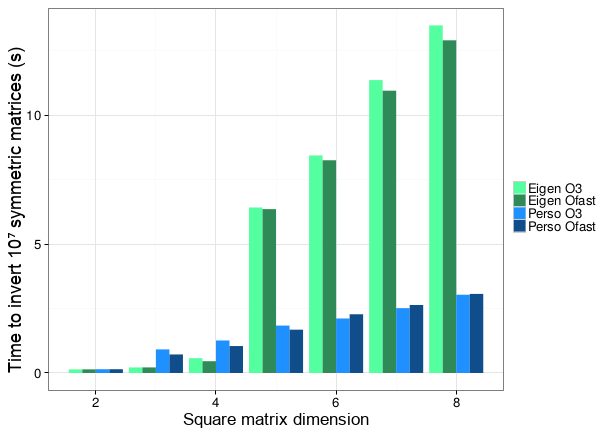
\includegraphics[scale=0.4]{Invert}
\centering
\end{figure}

Unfortunately, this substrate-specific low level code could not be integrated. I will aim to provide those improvements in a cross-platform manner. Specifically, I will investigate replacing the use of \texttt{Eigen} with the C++ library \texttt{xtensor}.\ \texttt{xtensor} aims to provide the functionality and feel of NumPy, a Python package with which HEP physicists are likely to be familiar, and may thus ease algorithmic contributions to the ACTS project. The threefold benefit of adopting it would thus be, more extensible code, potentially better cross-platform vectorisation, and room for my contribution of more effective algorithms for handling of small matrices, with emphasis on $5 \times 5$.

The latter objective has been mathematically neglected. $5 \times 5$ is the awkward boundary between the ubiquitous square matrices of smaller size carefully scrutinised by people working on computer graphics, and large matrices for which the primary consideration is asymptotics over constants.

\iffalse
\clearpage

Although long-lived particles carrying charge, such as electrons, may be accurately tracked,

Long lived particles carrying charge, such as electrons, may be accurately tracked.
The other 

as in the case of the Higgs boson, which has a mean lifetime of $10^{-22}$ s, 

However, other particles are too short lived to reach the detector walls,

In a collision experiment

Because some fundamental particles do not participate in certain interactions or do not carry charge, we can only infer that they were produced in a collision by looking at the terms missing from what we measure (e.g. in momentum and energy) and piecing together from which combination of undetectable particles this could arise.

One source of information is a reconstruction of paths taken by produced charged particles whilst moving through a strong magnetic field. ACTS is an open source library that performs such computations. These calculations involve frequent operation on $5 \times 5$ matrices, and most generally I would like to work on making them more efficient.

More specifically, in this particular use case, it arises that ACTS would perform a single operation independently on each member of a large set of matrices. Since 1975, when the Cray-1 supercomputer became the first to support vectorised instructions, processor architectures support operations performed on a sequence of memory locations - SIMD instructions.

In this project, I would adapt and optimise parts of the existing ACTS codebase to be written using the \texttt{xtensor} C++ library, which is specifically tailored to vectorised operations (and also lazy evaluation, which is not pertinent here). Algorithms written with excessive branching would need to be reconstructed to support vectorisation. Subsequently, I would work on benchmarking and cutting constants by reconsidering the mathematics that goes into the theory of $5 \times 5$ matrices, I being a mathematician in grad school. The project description page states that the $5 \times 5$ case has not already been scrutinised, it occurring less frequently then the ubiquitous square matrices of smaller size.

If \texttt{xtensor} is an effective choice for the ACTS codebase, then I would likely be able to contribute improvements to its handling of small matrices. Additionally, as I completing the qualifying task, I acquainted myself with \texttt{xtensor}, and noticed some other areas in which it could be improved. For example, its documentation in several sections and support of non-resizable views in \texttt{xtensorf} objects. Consequently, I would likely make several contributions to \texttt{xtensor} in the course of this project.

\section*{The Proposal}
\fi

\section*{Timescales, Purpose, and Deliverables}

Please note that the examination period of my current degree clashes for the first three weeks of the coding period. I believe that the remaining two months is sufficient to produce a substantial contribution, during which I will consider this a full time job. I however expect to be able to intimately familiarise myself with \texttt{xtensor} and the ACTS codebase prior to June 6\textsuperscript{th}.

The first deliverable would be an implementation of all that is involved in the Kalman filter algorithm, making effective use of the SIMD instruction capabilities provided by \texttt{xtensor}. I do not anticipate that producing clean and well documented code for this would take longer than a month, as I can identify a short list of the operations that I need to support, beyond which is a matter of negotiating with the library.

Subsequently, I would spend the rest of the project benchmarking, optimising, and considering the integration of this \texttt{xtensor} project into the ACTS code base proper. I expect that I would also make a mathematical contribution to constant cutting on some algorithms.

Finally, in the course of completing the qualifying task, I acquainted myself with \texttt{xtensor}. The documentation in several sections could be substantially improved. It would also be nice to let \texttt{xtensorf} objects support non-resizing views. Consequently, I may potentially make several contributions to \texttt{xtensor} in the course of this project.

\clearpage

\section*{My Background}

\begin{myparindent}{0pt}

\textsc{Undergraduate}: University of Waterloo, BMath in Pure Mathematics

\textsc{Master's}: University of Cambridge, MASt in Pure Mathematics (in progress)

\textsc{PhD}: Stony Brook University (starting in September)

\end{myparindent}

At Waterloo, my CS coursework consisted of:
\begin{itemize}
    \item Two semesters of freshman advanced computer science courses taught in Racket, a Lisp dialect.
    \item A course on object oriented design, C++, and the Unix command line.
    \item A basic compilers course, in which I wrote a rudimentary compiler for a C-like language in Racket. I have a half-finished reworking of this project currently in limbo, implementing optimisation through conversion to SSA form.
    \item An algorithms course, where I otherwise have done contest programming since high school.
    \item A course on real-time operating systems in my final term. My partner and I wrote a bare-metal embedded microkernel and operating system for controlling real life Märklin trains, this was primarily in C. For the kernell, we obsessed over excess optimisation of our scheduler and context switch (this was for an ARM4 processor), so I have spent a lot of time thinking about low level code.
\end{itemize}

Beyond coursework, I have frequently participated in Hackathons. Achievements include: `Most Functional' award at HackWaterloo in 2013. Finalist at WaterlooHacks in 2016. First place Wear Hacks KW 2017. My Devpost is: \href{https://devpost.com/Antares}{Antares}. I have used git for version control in both classes and hackathons.

My primary interest is mathematics. I have a strong background in analysis and topology/geometry. I completed eight graduate courses during my undergrad, presented as several conferences, and for the past three summers worked on research projects. I have one joint publication: \href{https://arxiv.org/abs/1711.09526}{[1711.09526]}.

I believe that my background makes me a strong match for this project because of the combined challenge of understanding and optimising code at a low level and the mathematical content. Peripherally, I have also studied as much physics as I have computer science and would be very happy to produce code that's used by researchers in experimental fundamental physics.

\clearpage

\section*{My Basic Information}

\begin{myparindent}{0pt}

\textsc{Email}: \texttt{tkolomatski@gmail.com}

\textsc{Homepage}: \href{http://csclub.uwaterloo.ca/~tkolomat/}{\url{http://csclub.uwaterloo.ca/~tkolomat/}}

\textsc{Nationality}: Canadian

\textsc{Timezones}: BST until July 1\textsuperscript{st}, then EDT

\textsc{Availability}: I have Part III exams during June 1-6. I will have significantly reduced availability prior to their end. Subsequently, I am free of any extended commitments.

\textsc{Permanent Mailing Address}:
\begin{align*}
    &\text{131 River Ridge Blcd.} \\
    &\text{Aurora, Ontario} \\
    &\text{L4G 7T7} \\
    &\text{Canada} \\
\end{align*}

\textsc{Emergency contact}: Tatiana Vichnitskaia (mother): \texttt{tvichnitskaia@hotmail.com}

\end{myparindent}

\end{document}
